% !TeX program = xelatex
\documentclass{scrartcl}

% This commad is defined in the makefile to generate the different
% language versions. If one compiles it directly this fallback is active.
\providecommand{\SelectedLanguage}{german}

% This commad is defined in the makefile to select a random color scheme.
% If one compiles it directly this fallback is active.
\providecommand{\SelectedColorSchemeNumber}{5}% = random

\RequirePackage{polyglossia}
   \setmainlanguage{\SelectedLanguage}

\usepackage{microtype}

\usepackage[
%   color-mode = gray,
   color-scheme-number = \SelectedColorSchemeNumber,
%   load-fonts = false,
]{citobiw}

\usepackage[
   language = \SelectedLanguage,
%   show-frame,
   year-format = YY,
]{cvtobiw}

\usepackage{hyperref}
   \urlstyle{same}

\newcommand{\softwareskills}{%
   Adobe CC (InDesign, InCopy,\linebreak Illustrator, Photoshop),
   Word, Excel, Powerpoint,
   Pages, Numbers, \mbox{Keynote},
   \TeX/,
   Terminal/Konsole,\linebreak
   Sibelius, Finale
}
\newcommand{\codingskills}{%
   \skill{\LaTeXe/}{90}\\
   \skill{\LaTeXiii/}{85}\\
   \skill{\TikZ/}{90}\\
   \skill{HTML\,5}{80}\\
   \skill{CSS\,3}{80}\\
   \skill{PHP}{70}\\
   \skill{Java/JavaScript}{40}
}
\newcommand{\osskills}{%
   \skill{Mac OS X}{100}\\
   \skill{Linux (Ubuntu)}{65}\\
   \skill{Windows}{45}
}

\newcommand{\projectlink}[1]{{% see german LaTeX Companion (LaTeX Begleiter; 2. ed.), p. 883
   \hspace*{\fill}%
   \nolinebreak[3]%
   \quad\hspace*{\fill}%
   \color{lightgray}%
   \finalhyphendemerits=0%
   \mbox{↗~\href{http://#1}{#1}}%
}}

\begin{document}

\begin{languagecontent}{german}
   \setvar{main}{%
      \textcp{\textbf{Hallo.}}
      
      Darf ich mich Ihnen vorstellen? Ich bin Tobias Weh, Lehrer und freier Grafiker
      aus Osnabrück. Neben der Physik und der Musik schlägt mein Herz vor allem für
      Buchstaben, Typografie und natürlich gute Gestaltung. \emph{Design} bedeutet
      für mich in erster Linie das Lösen von einem konkreten Problem, um damit Ihnen
      oder Ihren Kunden das Leben in gewisser Weise zu erleichtern – zum Beispiel
      durch eine schnell und einfach zu erfassende Darstellung von Informationen.
      Erst wenn so eine Lösung gefunden ist, kann man sie mit gestalterischen Mitteln
      und sauberem Handwerk in eine ästhetische Form bringen und damit eine
      nachhaltige und gute Gestaltung erreichen.
      
      Ich stehe Ihnen gerne zur Verfügung, um mit Ihnen gemeinsam ein
      Erscheinungsbild (\emph{Corporate Design}) zu entwickeln, für Ihre Texte
      oder Noten ein angemessenes Layout zu finden und sie zu setzen, für Ihr
      Buch anschauliche Abbildungen anzufertigen, Flyer oder Postkarten zu
      gestalten oder um Sie in allen Fragen rund um \TeX/ zu beraten.
      
      Herzliche Grüße\\
      Tobias Weh
   }

   \setvar{contact}{%
      T\kern-1ptobias W\kern-0.4pteh\\
      Spindelstraße 25\\
      40980 Osnabrück
      
      05\kern0.2pt4\kern-0.2pt1\,·\,40\kern-0.1pt757837\\
      0\kern-0.2pt160\,·\,5063337
      
      \href{mailto:mail@tobiw.de}{mail\raisebox{0.1ex}{@}tobiw\kern-0.75pt.de}\\
      \href{http://tobiw.de}{tobiw\kern-0.75pt.de}
   }

   \setvar{skills}{
      \minisec{Sprachen}
      \skill{Deutsch}{100}\\
      \skill{Englisch}{75}
      
      \minisec{Programme}
      \softwareskills
      
      \minisec{Programmiersprachen}
      \codingskills
      
      \minisec{Systeme}
      \osskills
   }

   \setvar{timeline-entries}{
      \timelineentry{1988}{geboren in Stadthagen bei Hannover}{}[28]
      \timelineentry{2007}{Abitur am Fachgymnasium Technik, Stadthagen}
         {Leistungskurse: Deutsch und\linebreak Elektrotechnik}
      \timelineentry{2007-2008}[14]{Freiwilliges Soziales Jahr Kultur}
         {Im Rahmen meines FSJ beim Landesmusikrat Niedersachsen e.\,V.
         habe ich diverse Projekte wie \emph{Jugend musiziert}
         mitorganisiert und durchgeführt.}[14]
      \timelineentry{2008-2014}{Studium an der Uni Osnabrück}
         {Lehramt für Gymnasium\\(Physik und Musik)}
      \timelineentry{2011-2014}[1]{\TeX/-Kurse}
         {im Fachbereich Physik\linebreak der Uni Osnabrück}
      \timelineentry{2012}[2]{Bachelorarbeit}
         {„Entwicklung des Java-Programms FIELDS zur zweidimensionalen\linebreak Darstellung
         von Feldern mithilfe des PhidgetInterfaceKit 2/2/2“}[11]
      \timelineentry{2014}[2]{Masterarbeit}
         {„Anschauliche Erklärung der trans\-mittierten und reflektierten Schallwellen
         am Ende einer offenen Röhre“}[11]
      \timelineentry{2011-today}[15]{selbstständige T\kern0.1ptätigkeit}
         {als Grafiker, Setzer, \TeX/-Berater}
      \timelineentry{2012-2014}[16]{wissenschaftliche Hilfskraft}
         {Betreuung der Internetseite (Typo3)\linebreak des Instituts für Musik der\linebreak Uni Osnabrück}
      \timelineentry{2013-mid2013}[17]{wissenschaftliche Hilfskraft}
         {Tutor in der Physikdidaktik an der Uni Osnabrück}[10]
      \timelineentry{2014-today}[17]{Studium an der FH Bielefeld}
         {Bachelor Gestaltung\\(Grafik und Kommunikationsdesign)}
   }

   \setvar{code}{
      Erstellt mit \TeX/ – Code auf \href{https://github.com/tweh/cv}{github.com/tweh/cv}.
   }
\end{languagecontent}

\begin{languagecontent}{english}
   \setvar{main}{%
      \textcp{\textbf{Hello.}}
      
      May I introduce myself? I am Tobias Weh, teacher and freelancing graphic
      designer from Osnabrueck (Germany). Besides physics and music I love
      letters, typography and of course great design. For me \emph{design}
      basically means solving problems in order to help making your or your
      client’\kern-0.5pts life a bit easier – for example by providing
      information in a structured and legible manner. If such a solution is
      found one can start to style it by using the methods of design and craft
      to make it appealing.
      
      I am available for creating a new corporate design for you, finding a proper
      layout for your texts and music scores, illustrating your book, designing
      flyers and posters, or helping you with all questions regarding \TeX/.
      
      Yours sincerely\\
      Tobias Weh
   }
   
   \setvar{timeline-entries}{
      \timelineentry{1988}{Born in Stadthagen near Hannover}{}[28]
      \timelineentry{2007}{Abitur (\textit{GCE A-levels}) at Fachgymnasium Technik
         (\textit{technical upper secondary school}), Stadthagen}{}
      \timelineentry{2007-2008}[14]{Voluntary Social Year}
         {During my voluntary social year at the Lower-Saxony Music Council
         I helped planing and organizing projects like \emph{Jugend musiziert}
         (\emph{young musician competition}).}[14]
      \timelineentry{2008-2014}{Study at the University of\linebreak Osnabrueck}
         {Secondary school teacher \linebreak (physics and music)}
      \timelineentry{2011-2014}[1]{\TeX/ Tutorials}
         {at the physics department of the University of Osnabrueck}
      \timelineentry{2012}[2]{Bachelor Thesis}
         {Developing a software to measure two dimensional fields with the
         PhidgetInterfaceKit 2/2/2}[11]
      \timelineentry{2014}[2]{Master Thesis}
         {Descriptive explanation of transmitted and reflected sound waves at the
         open end of a tube.}[11]
      \timelineentry{2011-today}[15]{Freelancer}
         {as designer, typesetter, and\linebreak \TeX/ consultant}
      \timelineentry{2012-2014}[16]{Research Assistant}
         {Maintenance of the homepage (Typo3) of the music department of
         the University of Osnabrueck}
      \timelineentry{2013-mid2013}[17]{Research Assistant}
         {Tutor for didactics of physics at the University of\linebreak Osnabrueck}[10]
      \timelineentry{2014-today}[17]{Study at the University of Applied Science Bielefeld}
         {Bachelor in design\linebreak (graphic and communication design)}
   }
   
   \setvar{contact}{%
      T\kern-1ptobias W\kern-0.4pteh\\
      Spindelstrasse 25\\
      40980 Osnabrueck\\
      Germany\\[0.5\baselineskip]
      %
      +49\,5\kern0.2pt4\kern-0.2pt1\,·\,40\kern-0.1pt757837\\
      +49\,160\,·\,5063337\\[0.5\baselineskip]
      %
      \href{mailto:mail@tobiw.de}{mail\raisebox{0.1ex}{@}tobiw\kern-0.75pt.de}\\
      \href{http://tobiw.de}{tobiw\kern-0.75pt.de/\kern-0.5pten}
   }

   \setvar{skills}{
      \minisec{Languages}
      \skill{German}{100}\\
      \skill{English}{80}
      
      \minisec{Software}
      \softwareskills
      
      \minisec{Programming Languages}
      \codingskills
      
      \minisec{Operating Systems}
      \osskills
   }

   \setvar{code}{
      Made with \TeX/ – Code at \href{https://github.com/tweh/cv}{github.com/tweh/cv}
   }
\end{languagecontent}

\setvar{image}{
   \includegraphics[width=\usedim{right-col-width}]{img/tobiw}
}

\setvar{logo}{
   \TobiWLogo[height=4ex]
}

\setvar{timeline-birth}{1988}
\setvar{timeline-start}{2007}
\setvar{timeline-end}{2015}

\MakeCV

% ============================================================

\newproject{dekonstruiert}
\newproject{master}
\newproject{metrix}
\newproject{mos}
\newproject{musicaincantans}
\newproject{nve}
\newproject{speight}

\begin{languagecontent}{german}
   \setprojectvar{dekonstruiert}{title}{Dekonstruiert}
   \setprojectvar{dekonstruiert}{content}{
      Das Büchlein \emph{Dekonstruiert} nimmt den Leser mit auf eine „Reise ins
      Detail“ und beleuchtet dabei die verschiedensten Aspekte der Buchproduktion vom
      Satzspiegel, über das Druckraster bis hin zu Quanten. Das Büchlein habe ich mit
      Illustrator und InDesign erstellt.
      \projectlink{tobiw.de/illustration}
   }
   
   \setprojectvar{master}{title}{Transmittierte und reflektierte Wellen}
   \setprojectvar{master}{content}{
      Zum Abschluss meines Lehramtsstudiums entstand meine Masterarbeit mit dem Titel
      „Anschauliche Erklärung der trans\-mittierten und reflektierten Schallwellen am
      Ende einer offenen Röhre“. Die Arbeit habe ich mit \XeTeX/ gesetzt und mit \TikZ/
      \linebreak illustriert.
      \projectlink{tobiw.de/galerie/schwingungen-und-wellen}
   }
   
   \setprojectvar{metrix}{title}{\LaTeX/-Paket \emph{metrix}}
   \setprojectvar{metrix}{content}{
      Das Paket \emph{metrix} dient dazu die Prosodie eines (lateinischen) Verses
      anzugeben, wobei die Ausrichtung der Symbole über den Silben halbautomatisch
      erfolgt. Das Paket habe ich weitestgehend mit den neuen \LaTeXiii/-Funktionen
      implementiert.
      \projectlink{tobiw.de/tex-beratung-und-programmierung\#metrix}
   }
   
   \setprojectvar{mos}{title}{Musikedition Osnabrücker Schloss}
   \setprojectvar{mos}{content}{
      Für die 2013 gegründete Reihe für kritische Ausgaben von Noten
      \emph{Musikedition Osnabrücker Schloss} habe ich ein Layout ausgearbeitet und
      den Satz der bisher erschienenen Ausgaben übernommen. Bei der ersten Ausgabe
      war ich außerdem an der\linebreak Edition selbst beteiligt.
      \projectlink{tobiw.de/notensatz}
   }
   
   \setprojectvar{musicaincantans}{title}{Musica Incantans}
   \setprojectvar{musicaincantans}{content}{
      \emph{Musica Incantans} ist die kritische Ausgabe eines neulateinischen
      Gedichtes von Robert South über die Macht der Musik. Das Gedicht selbst ist auf
      gegenüberliegenden Seiten im Original und in deutscher Übersetzung gedruckt.
      Gesetzt habe ich es mit \XeTeX/.
      \projectlink{tobiw.de/buch-und-textgestaltung}
   }
   
   \setprojectvar{nve}{title}{Niedersächsisches Vokalensemble e.\,V.}
   \setprojectvar{nve}{content}{
      Das Niedersächsisches Vokalensemble ist ein 2014 ins Leben gerufener,
      Kammerchor, der anspruchsvolle Chormusik von der Renaissance bis zur
      Moderne aufführt. Ich habe für den Chor ein Corporate Design entwickelt
      und in verschiedenen Medien umgesetzt.
      \projectlink{tobiw.de/corporate-design}
   }
   
   \setprojectvar{speight}{title}{Sam\kern-0.2pt’\kern-0.7pts Mass}
   \setprojectvar{speight}{content}{
      Für den Kammerchor der Uni Osnabrück habe ich aus den nur in Handschrift
      erhältlichen Noten von \emph{Sam’\kern-0.6pts Mass} eine leichter lesbare
      gedruckte Version angefertigt, wobei ich zusätzliche Symbole entwickelt
      habe, um den Sängern die Orientierung zu erleichtern.
      \projectlink{tobiw.de/en/gallery/sams-mass}
   }
\end{languagecontent}

\begin{languagecontent}{english}
   \setprojectvar{dekonstruiert}{title}{Dekonstruiert}
   \setprojectvar{dekonstruiert}{content}{
      The booklet \emph{Dekonstriert} (\emph{Deconstructed}) invites the reader to take
      a journey through all aspects of book design and production. Some of the
      topics are page layout, printing but also atoms, quarks and strings.
      I made the booklet with Illustrator and InDesign.
      \projectlink{tobiw.de/en/illustration}
   }
   
   \setprojectvar{master}{title}{Transmitted and reflected waves}
   \setprojectvar{master}{content}{
      At the end of my studies in Osnabrueck I wrote my master thesis about finding
      a descriptive explanation of transmitted and reflected sound waves at the
      open end of a tube. The thesis was typeset with \XeTeX/ and illustrated
      with \TikZ/.
      \projectlink{tobiw.de/en/gallery/oscillations-and-waves}
   }
   
   \setprojectvar{metrix}{title}{\LaTeX/ package \emph{metrix}}
   \setprojectvar{metrix}{content}{
      The package \emph{metrix} can be used to typeset metric
      symbols above (latin) verses with a semi-automatic alignment above the syllables.
      I mainly used the new \LaTeXiii/ syntax to code the package.
      \projectlink{tobiw.de/en/tex-consulting-and-programming\#metrix}
   }
   
   \setprojectvar{mos}{title}{Musikedition Osnabrücker Schloss}
   \setprojectvar{mos}{content}{
      The series \emph{Musikedition Osnabrücker Schloss} (\emph{Music Edition
      Castle of Osnabrueck}) was started in 2013 and I designed a layout and
      typeset the already published volumes. Furthermore, I participated in the
      editorial work of the first volume.
      \projectlink{tobiw.de/en/music-typesetting}
   }
   
   \setprojectvar{musicaincantans}{title}{Musica Incantans}
   \setprojectvar{musicaincantans}{content}{
      \emph{Muscia Incantans} is the critical edition, translation, and
      accompanying commentary of a neo-latin poem by Robert South about the
      power of music. The poem is printed in Latin and German on facing pages. I
      typeset the book with \XeTeX/.
      \projectlink{tobiw.de/buch-und-textgestaltung}
   }
   
   \setprojectvar{nve}{title}{Niedersächsisches Vokalensemble e.\,V.}
   \setprojectvar{nve}{content}{
      The Niedersächsische Vokalensemble (Lower-Saxony Vocal Ensemble) is a
      chamber choir founded in 2014, to perform sophisticated choir music from
      the Renaissance to the Modern Era. I~developed a complete corporate design
      and implemented it for different media.
      \projectlink{tobiw.de/en/corporate-design}
   }
   
   \setprojectvar{speight}{title}{Sam\kern-0.2pt’\kern-0.7pts Mass}
   \setprojectvar{speight}{content}{
      For the chamber choir of the University of Osnabrueck I typeset
      \emph{Sam’\kern-0.6pts Mass} since the piece is only available handwritten
      and not that legible. My version also contains symbols to indicate changes
      in stave numbers to help the singers finding the right stave at a break.
      \projectlink{tobiw.de/en/gallery/sams-mass}
   }
\end{languagecontent}

\setprojectvar{dekonstruiert}{image}{
   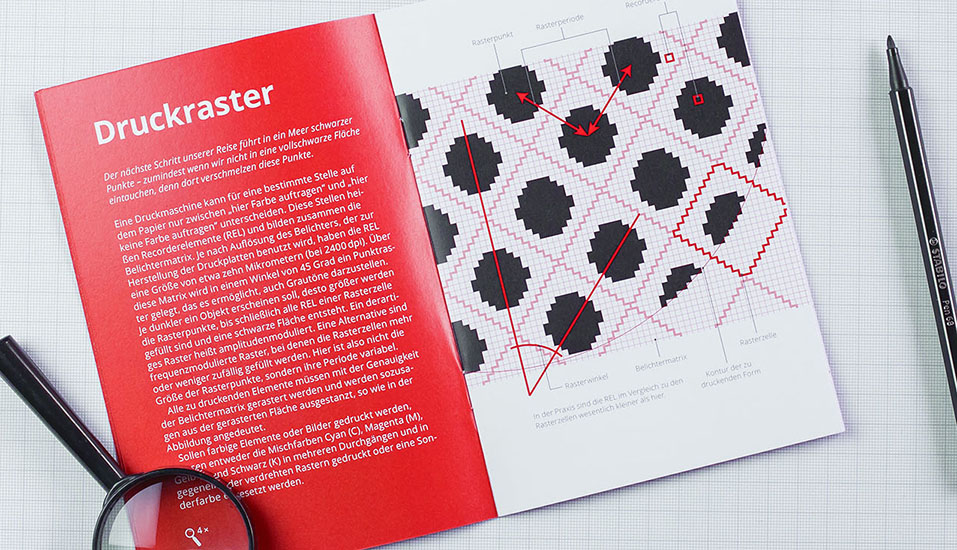
\includegraphics[width=\usedim{eq-col-width}]{img/projects/dekonstruiert}
}
\setprojectvar{master}{image}{
   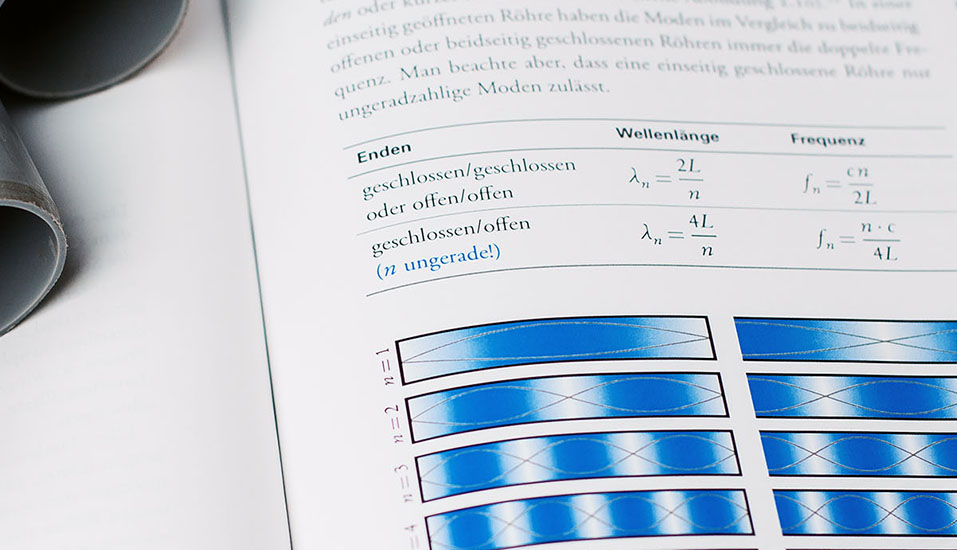
\includegraphics[width=\usedim{eq-col-width}]{img/projects/master_thesis}
}
\setprojectvar{metrix}{image}{
   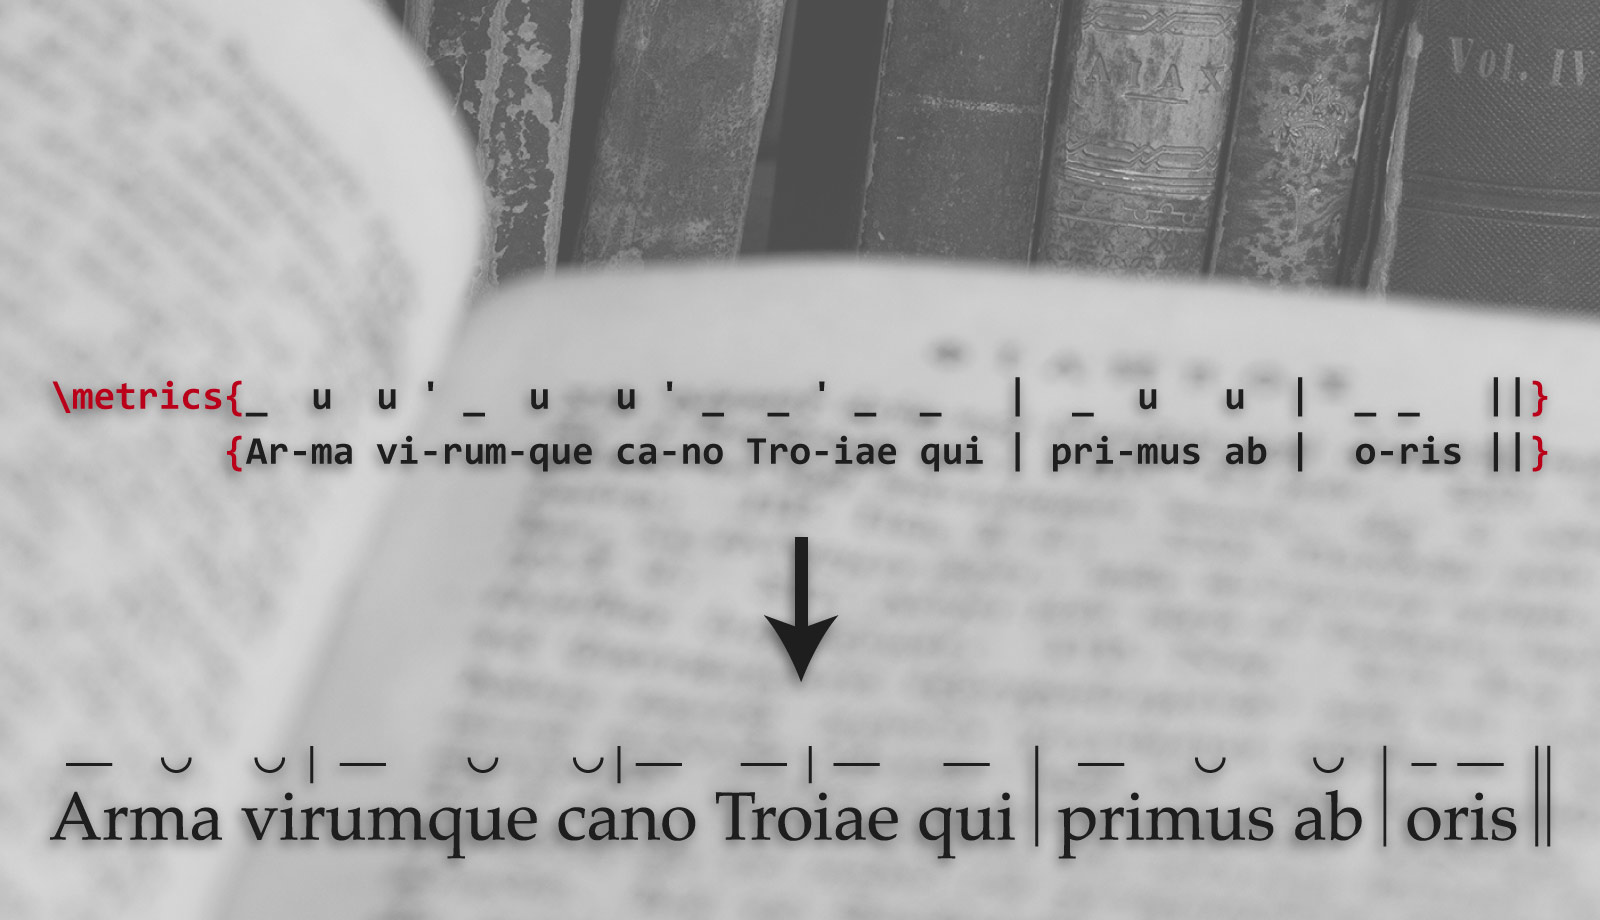
\includegraphics[width=\usedim{eq-col-width}]{img/projects/metrix}
}
\setprojectvar{mos}{image}{
   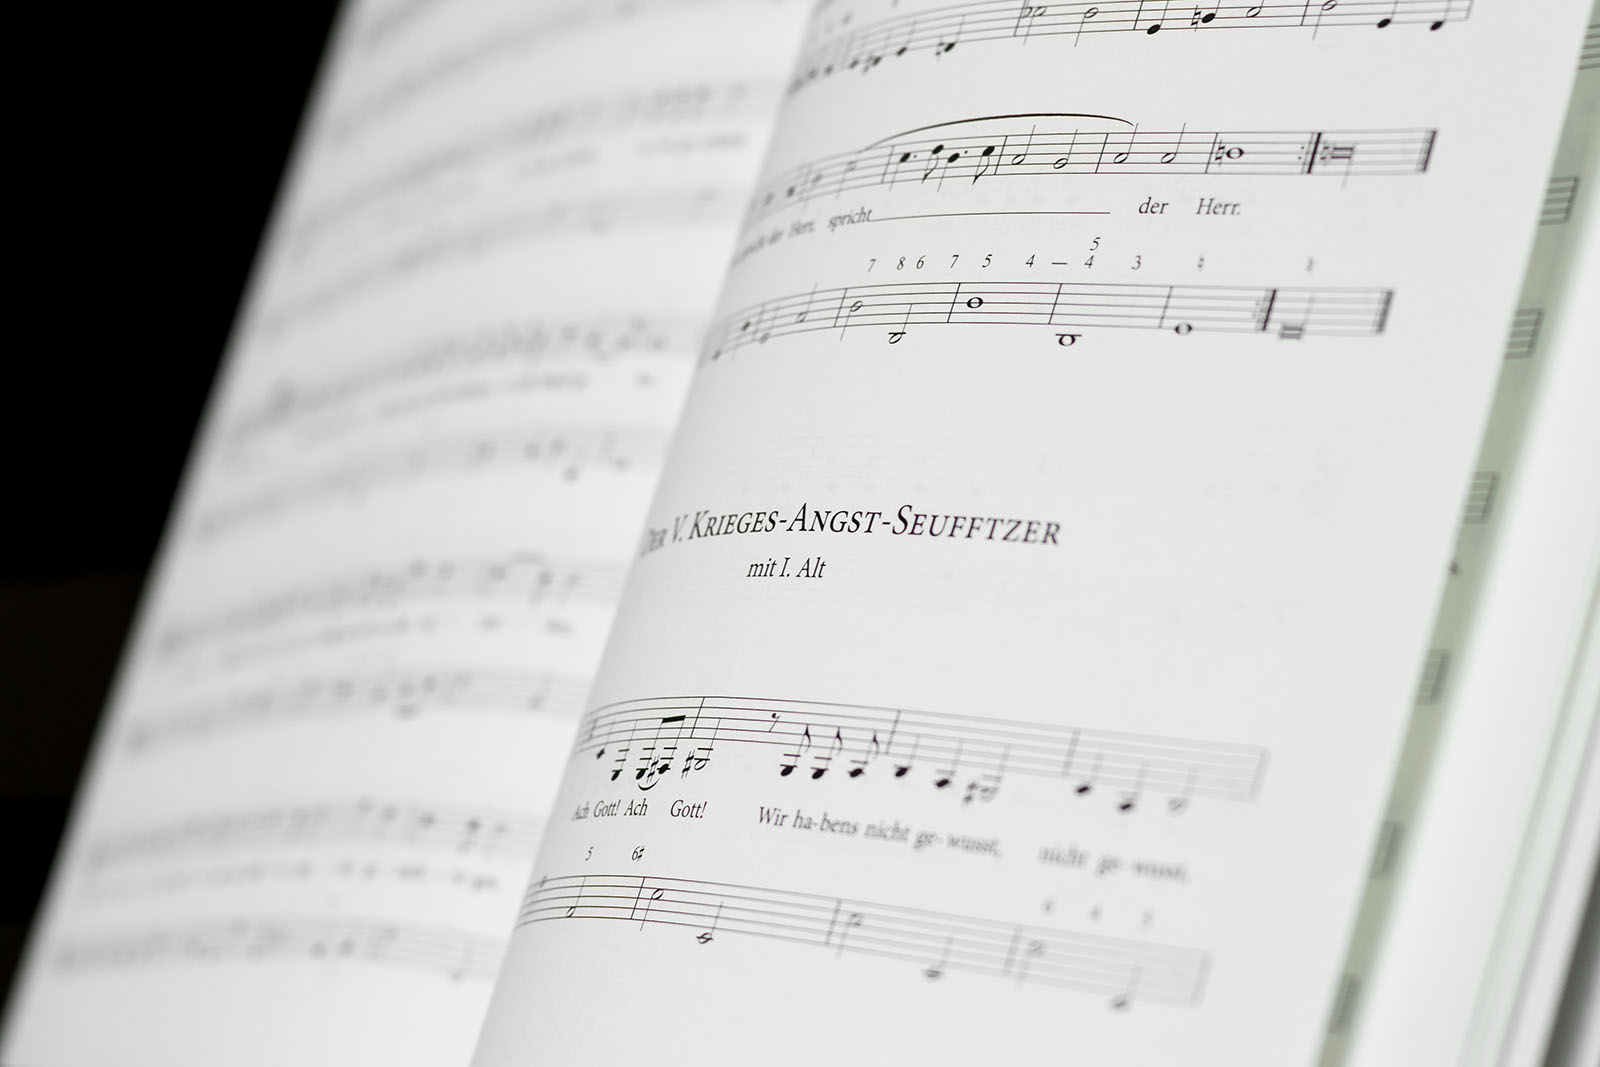
\includegraphics[width=\usedim{eq-col-width}]{img/projects/mos}
}
\setprojectvar{musicaincantans}{image}{
   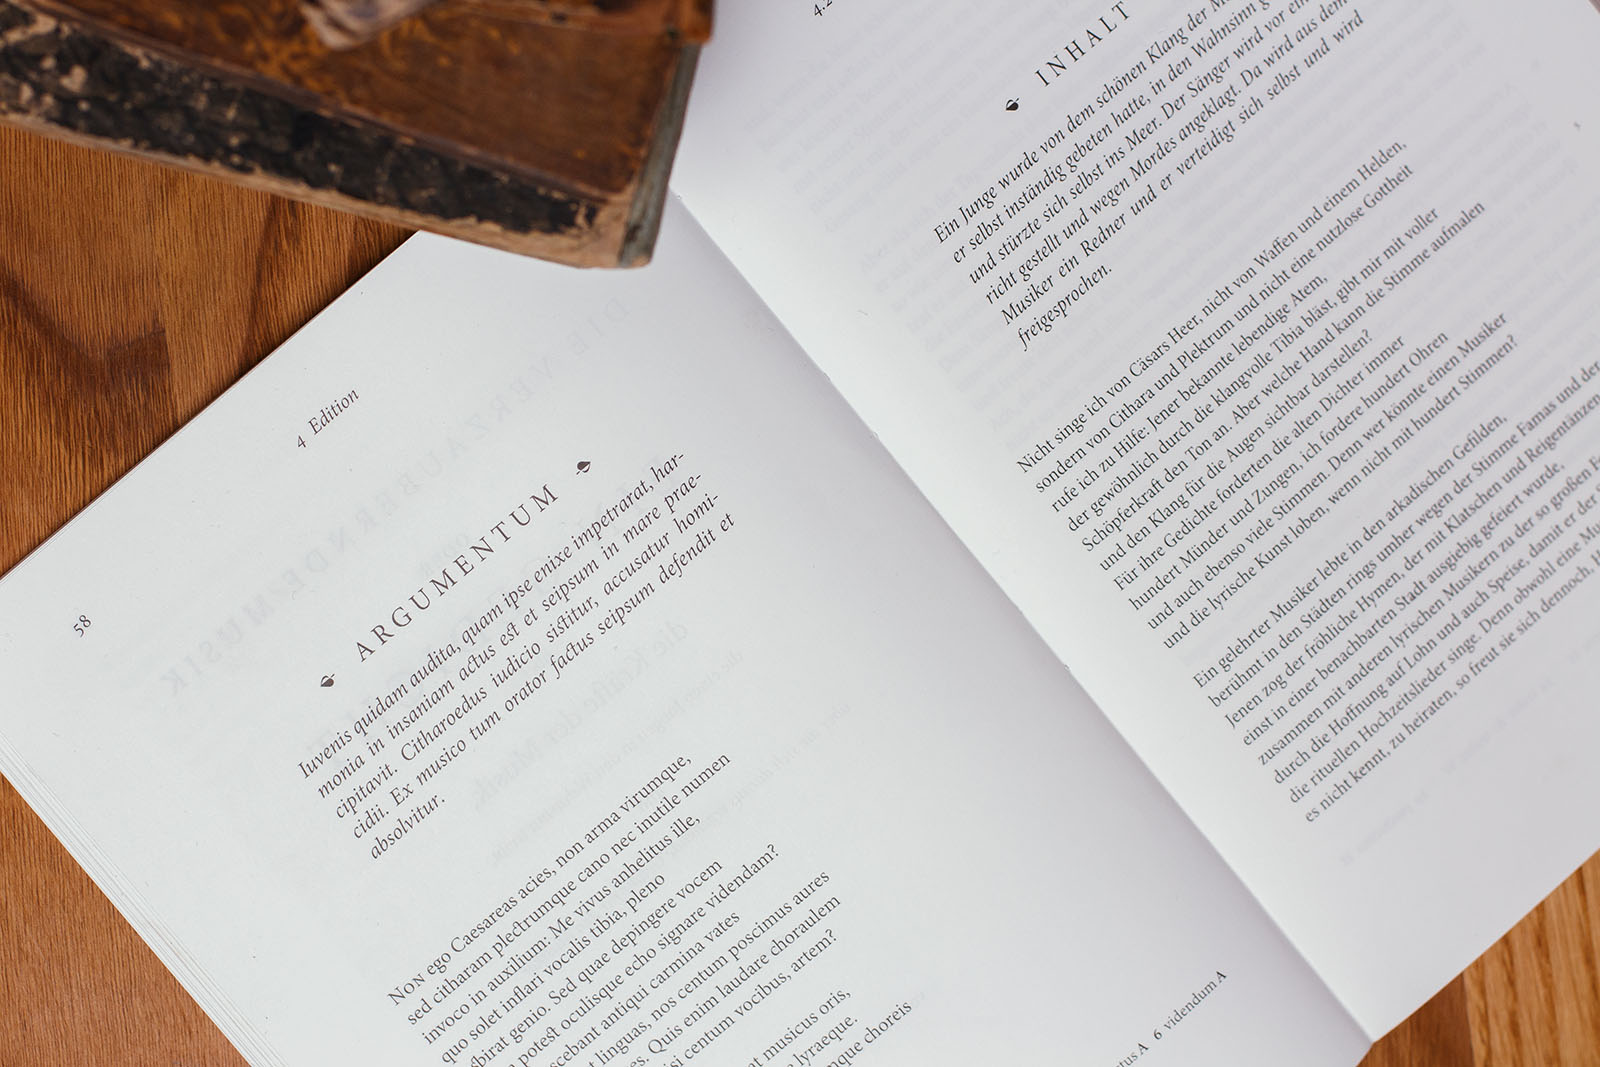
\includegraphics[width=\usedim{eq-col-width}]{img/projects/musica_incantans}
}
\setprojectvar{nve}{image}{
   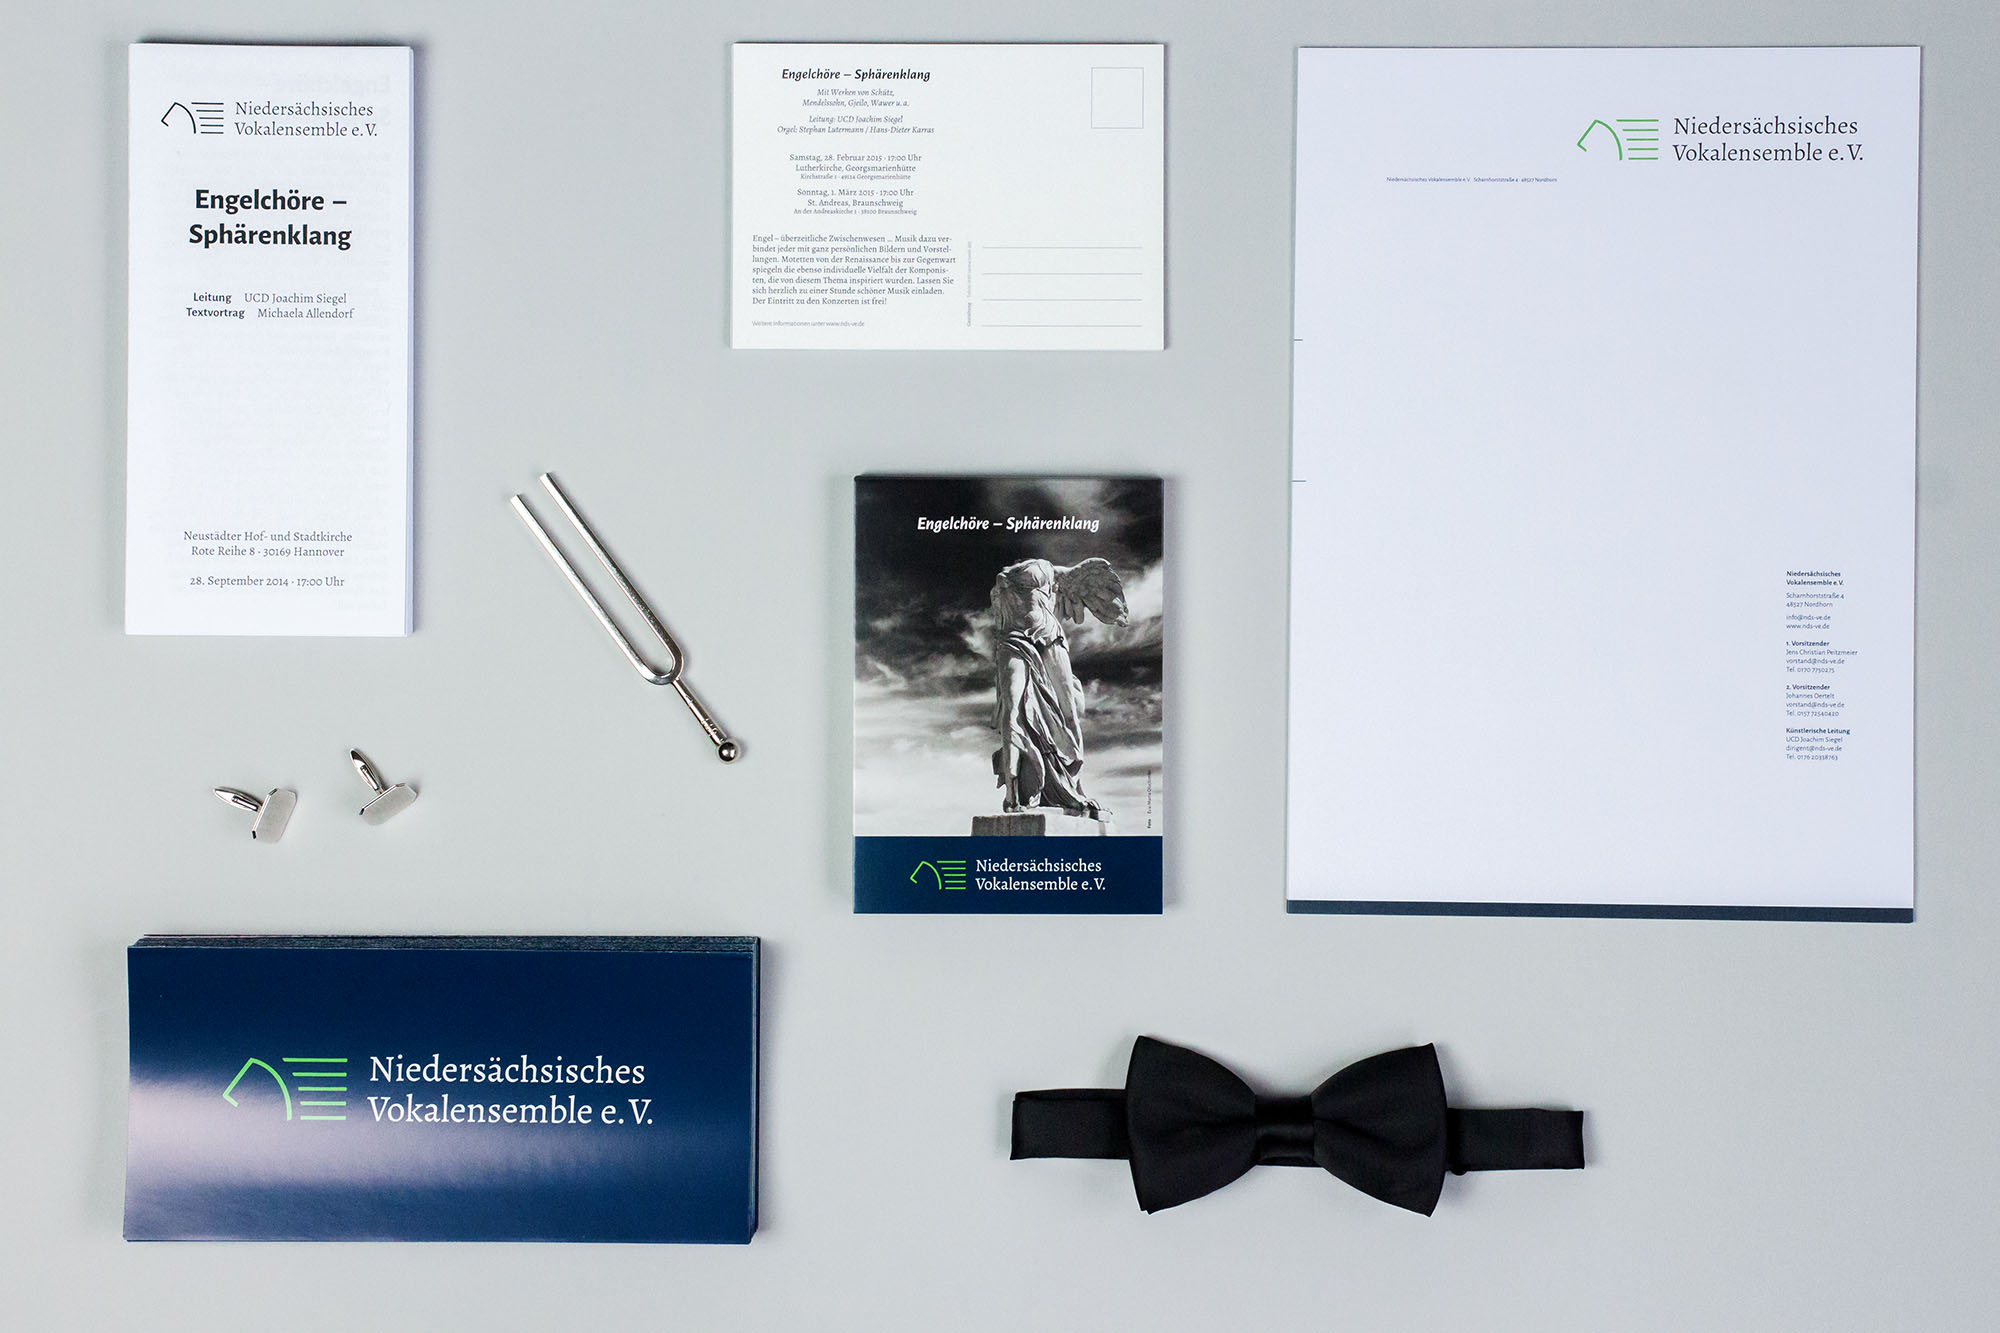
\includegraphics[width=\usedim{eq-col-width}]{img/projects/nve}
}
\setprojectvar{speight}{image}{
   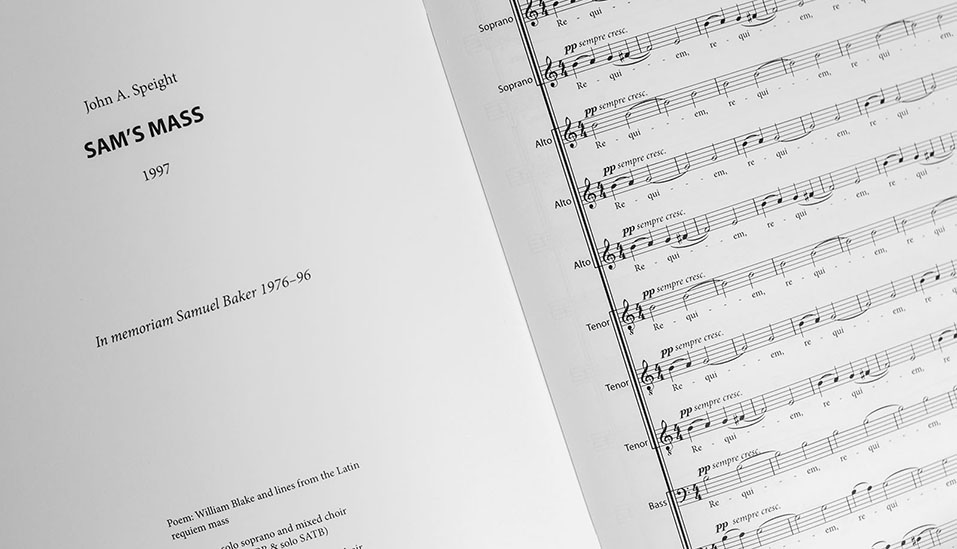
\includegraphics[width=\usedim{eq-col-width}]{img/projects/speight}
}

\MakePortfolio[
   dekonstruiert,
   nve,
   musicaincantans,
   metrix,
   master,
   mos%,
%   speight
]

\end{document}